
\begin{frame}
 \frametitle{Vectors}

\begin{itemize}
 \item Location of projector from current position and orientation:

\pause
\begin{itemize}
  \item direction of projector
  \item distance to projector
\end{itemize}

\pause
\item (direction, distance=magnitude) $\Longleftrightarrow$ \textit{vector}

\pause
\item Examples:
\begin{itemize}
  \item Force
  \item Velocity
  \item Displacement
\end{itemize}
\end{itemize}

\end{frame}

\begin{frame}
 \frametitle{Displacement Vectors}

\pause
  Displacement vector = ordered pair of points, $(A,B)$


\begin{itemize}
 \item Represented as an arrow
 \item $A$: tail, $B$: head
 \item Notation: $(A,B) = \overrightarrow{AB} = \textbf{AB}$
  \item Magnitude: $|\textbf{AB}| = |\overrightarrow{AB}|$. 
  \item Direction: Geometric direction from $A$ to $B$, if $A\neq B$ 
  \item If $A=B$:
  \begin{itemize}
    \item Zero magnitude and non-specified direction
    \item $(A,A) = \overrightarrow{AA} = \textbf{AA}$: zero displacement vector.
  \end{itemize}
  \item Displacement vector with tail fixed at $O$:
  \begin{itemize}
    \item Position vector with respect to $O$;
    \item $(O,P) = \overrightarrow{OP} = \textbf{OP} = \textbf{r}_P$.
  \end{itemize}
\end{itemize}

\end{frame}

\begin{frame}
 \frametitle{Equality and Equivalence of Displacement Vectors}

  \begin{itemize}
   \item Equality of displacement vectors: \pause
    $$\textbf{AB} = \textbf{DC} \Longleftrightarrow (A,B) = (D,C) \Longleftrightarrow A=D \text{ and } B=C$$
    \begin{itemize}
      \item Useful for position vectors:
      $$\textbf{OP} = \textbf{OQ} \Longleftrightarrow P=Q\; .$$
      \item In general too restrictive. \pause
    \end{itemize}
    \item Equal displacement vectors $\rightarrow$ same magnitude and direction.
    \item Same magnitude and direction $\not\rightarrow$ Equal displacement vectors. \pause
    \item  Equivalent displacement vectors $\Leftrightarrow$ Same magnitude and direction
    $$\textbf{AB} \equiv \textbf{DC} \Longleftrightarrow ABCD \text{ is a parallelogram}\;.$$
  \end{itemize}

\end{frame}

\begin{frame}
 \frametitle{Vectors}

  \begin{itemize}
   \item Vector $\textbf{u}$: \\
      set of displacement vectors with given direction and magnitude

    \item  Magnitude of $\textbf{u}$: common given magnitude.

    \item Direction of $\textbf{u}$: common given direction, if non-zero magnitude.

    \item Set of zero displacement vectors = zero vector, $\textbf{0}$. \pause

    \item Representative for $\textbf{u}$: \\
      displacement vector $\textbf{AB}$ with the same direction and magnitude

\begin{figure}[h]
  \psfrag{A}{$A$}
  \psfrag{B}{$B$}
  \psfrag{C}{$C$}
  \psfrag{D}{$D$}
  \psfrag{E}{$E$}
  \psfrag{F}{$F$}
  \psfrag{u}{$\textbf{u}$}
  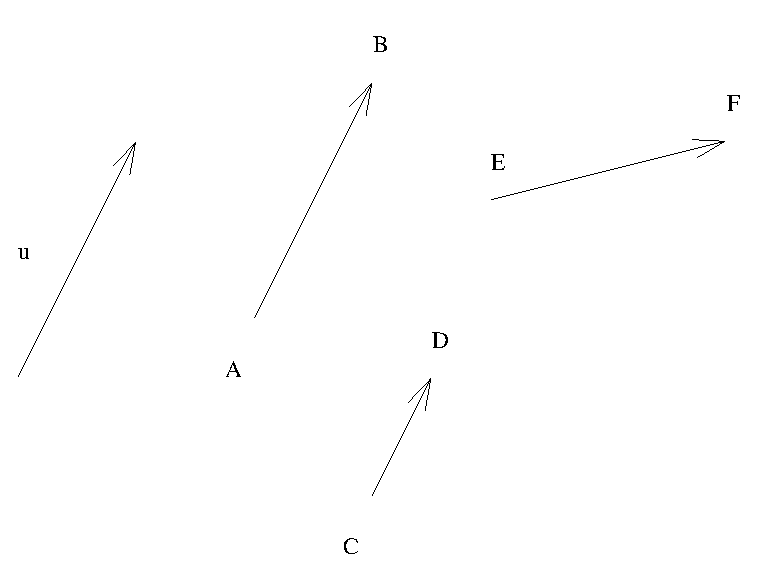
\includegraphics[height=1in]{../images/ok-vector_representatives.eps}
  \label{fig:vector_representative}

\end{figure}

    \item Intuitive notation:  $\textbf{u}=\textbf{AB}$.

    \item Graphical representation: arrow without fixed tail and head.

    %\item Major advantage: we can translate displacement vectors.
  \end{itemize}
\end{frame}

\begin{frame}
 \frametitle{Addition of Vectors}

  \begin{itemize}
    \item By adding representative displacement vectors: Triangle Rule
\only<2>{
\begin{figure}[h]
  \psfrag{A}{$A$}
  \psfrag{B}{$B$}
  \psfrag{C}{$C$}
  \psfrag{P}{$P$}
  \psfrag{Q}{$Q$}
  \psfrag{R}{$R$}
  \psfrag{u}{$\textbf{u}$}
  \psfrag{v}{$\textbf{v}$}
  \psfrag{uv}{$\textbf{u}+\textbf{v}$}
  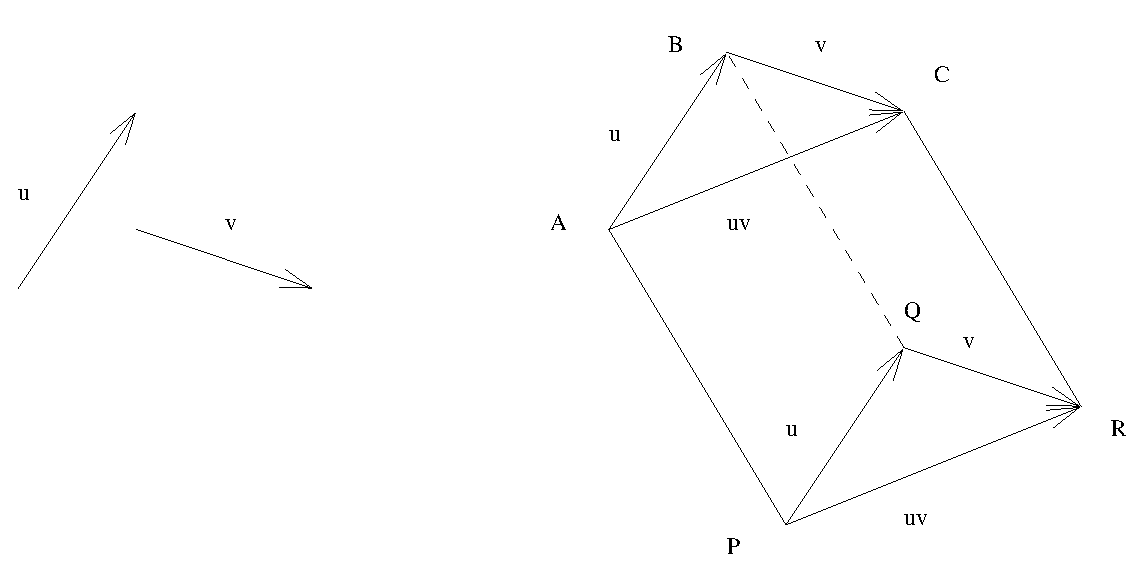
\includegraphics[height=1in]{../images/ok-vector_addition.eps}
  \label{fig:vector_addition}
  %\caption{Sum of two vectors}
\end{figure}}
    \item<3-> Properties:
    \begin{itemize}
      \item<4-> Commutative, $\textbf{u}+\textbf{v}$ = $\textbf{v}+\textbf{u}$ : Parallelogram Rule
\only<5, 10>{
\begin{figure}[h]
  \psfrag{A}{$A$}
  \psfrag{B}{$B$}
  \psfrag{C}{$C$}
  \psfrag{D}{$D$}
  \psfrag{u}{$\textbf{u}$}
  \psfrag{v}{$\textbf{v}$}
  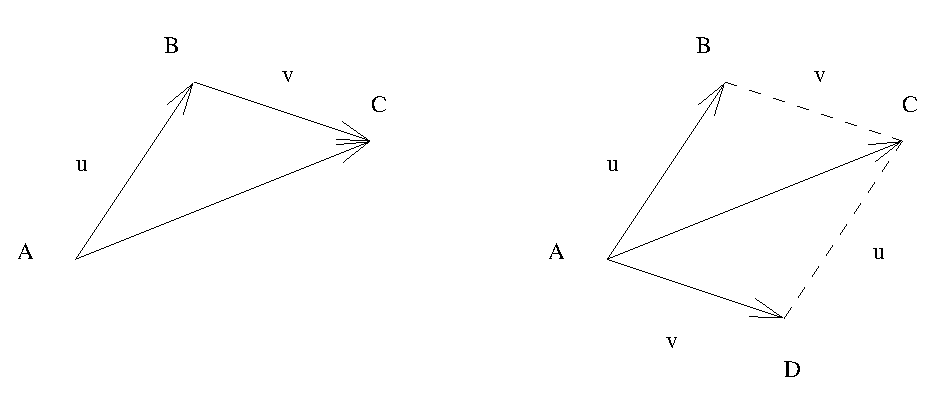
\includegraphics[height=1in]{../images/ok-tri-para_rules.eps}
  \label{fig:tripara_rules}
  %\caption{Triangle and Parallelogram Rules}
\end{figure}}

      \item<6-> Associative, $(\textbf{u}+\textbf{v})+\textbf{w} = \textbf{u}+(\textbf{v}+\textbf{w})$ \\
      Extends addition to $\textbf{u}+\textbf{v}+\textbf{w}$
\only<7>{
\begin{figure}[h]
  \psfrag{A}{$A$}
  \psfrag{B}{$B$}
  \psfrag{C}{$C$}
  \psfrag{D}{$D$}
  \psfrag{u}{$\textbf{u}$}
  \psfrag{v}{$\textbf{v}$}
  \psfrag{w}{$\textbf{w}$}
  \psfrag{uv}{$\textbf{u}+\textbf{v}$}
  \psfrag{vw}{$\textbf{v}+\textbf{w}$}
  \psfrag{uvw}{$\textbf{u}+\textbf{v}+\textbf{w}$}
  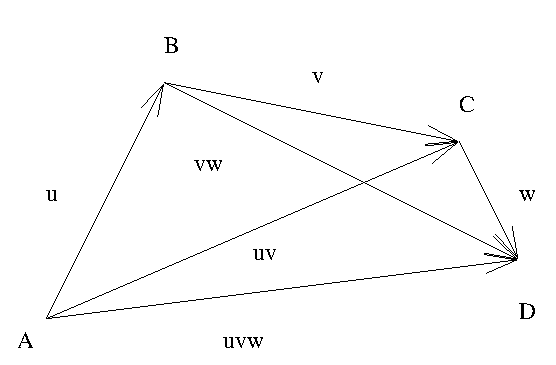
\includegraphics[height=1.5in]{../images/ok-assoc_addition.eps}
  \label{fig:assoc_adition}
  %\caption{Sum of three vectors}
\end{figure}}

      \item<8-> Opposite vector: If $\textbf{u}=\textbf{AB}$, then $\textbf{AB} + \textbf{BA} = \textbf{0}$,
      hence $\textbf{BA} = -\textbf{u}$.
    \end{itemize}
    \item<9-> Difference of vectors: $\textbf{u}-\textbf{v} = -\textbf{v}+\textbf{u}\textbf{}$: Parallelogram rule.

  \end{itemize}

\end{frame}

\begin{frame}
 \frametitle{Linear Combinations}

\begin{itemize}
 \item Scalar multiples: Let $\textbf{u}$ be a vector and $c$ a real number (scalar)
  \begin{itemize}
    \item If $c >0$ then $c\textbf{u}$ is the vector: \pause
    \begin{itemize}
      \item with the same direction
      \item with magnitude $|c\textbf{u}| = c|\textbf{u}|$.
    \end{itemize}\pause
     \item If $c<0$ then $c\textbf{u} = (-c)(-\textbf{u})$: \pause
     \begin{itemize}
	\item opposite direction
	\item magnitude $|c\textbf{u}| = |(-c)(-\textbf{u})| = (-c)|-\textbf{u}| = |c||\textbf{u}|$
     \end{itemize}\pause
     \item If $c=0$ then \pause $c\textbf{u} = \textbf{0}$. \pause
  \end{itemize}
  \item If $c_1, \ldots , c_n$ are scalars and $\textbf{u}_1,\ldots,\textbf{u}_n$ are vectors, then
%
$$\textbf{v} = c_1\textbf{u}_1+ \dotsb + c_n \textbf{u}_n$$
%
is the linear combination of given vectors with given scalars.
\end{itemize}

\end{frame}

\begin{frame}
  \frametitle{Decomposition of a vector along given directions}

  Example: Tension induced by given force.

\begin{figure}[h]
  \psfrag{F}{$\textbf{F}$}
  \psfrag{-F}{$-\textbf{F}$}
  \psfrag{F1}{$\textbf{F}_1$}
  \psfrag{F2}{$\textbf{F}_2$}
  \psfrag{T1}{$\textbf{T}_1$}
  \psfrag{T2}{$\textbf{T}_2$}
  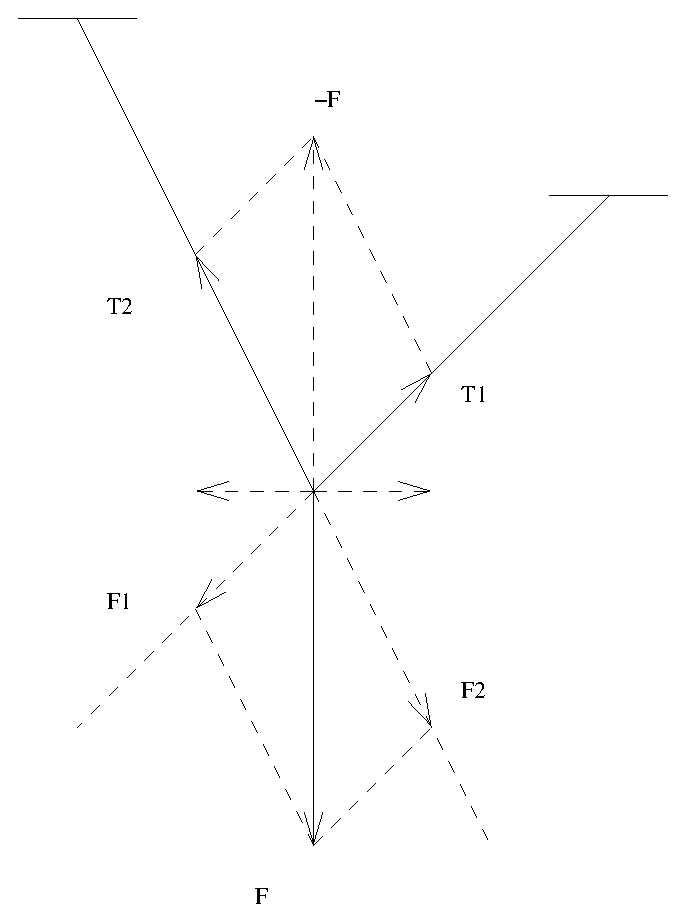
\includegraphics[height=2in]{../images/ok-tension.eps}
  \label{fig:tension}
  %\caption{Decomposition of a vector}
\end{figure}


\end{frame}

\begin{frame}
 \frametitle{Vectors in Coordinates}

  \begin{itemize}
    \item $Oxyz$: fixed rectangular coordinate system
    \item $\textbf{i}$, $\textbf{j}$, $\textbf{k}$: unit vectors in the fundamental directions
  \end{itemize}

If $P(a,b,c)$ is a point, then
\begin{figure}[h]
  \psfrag{a}{$a$}
  \psfrag{b}{$b$}
  \psfrag{c}{$c$}
  \psfrag{x}{$x$}
  \psfrag{y}{$y$}
  \psfrag{z}{$z$}
  \psfrag{ai}{$a \textbf{i}$}
  \psfrag{bj}{$b \textbf{j}$}
  \psfrag{ck}{$c \textbf{k}$}
  \psfrag{i}{$\textbf{i}$}
  \psfrag{j}{$\textbf{j}$}
  \psfrag{k}{$\textbf{k}$}
  \psfrag{P}{$P(a,b,c)$}
  \psfrag{Px}{$P_x(a,0,0)$}
  \psfrag{Py}{$P_y(0,b,0)$}
  \psfrag{Pz}{$P_z(0,0,c)$}
  \psfrag{Pxy}{$P_{xy}(a,b,0)$}
  \psfrag{O}{$O$}
  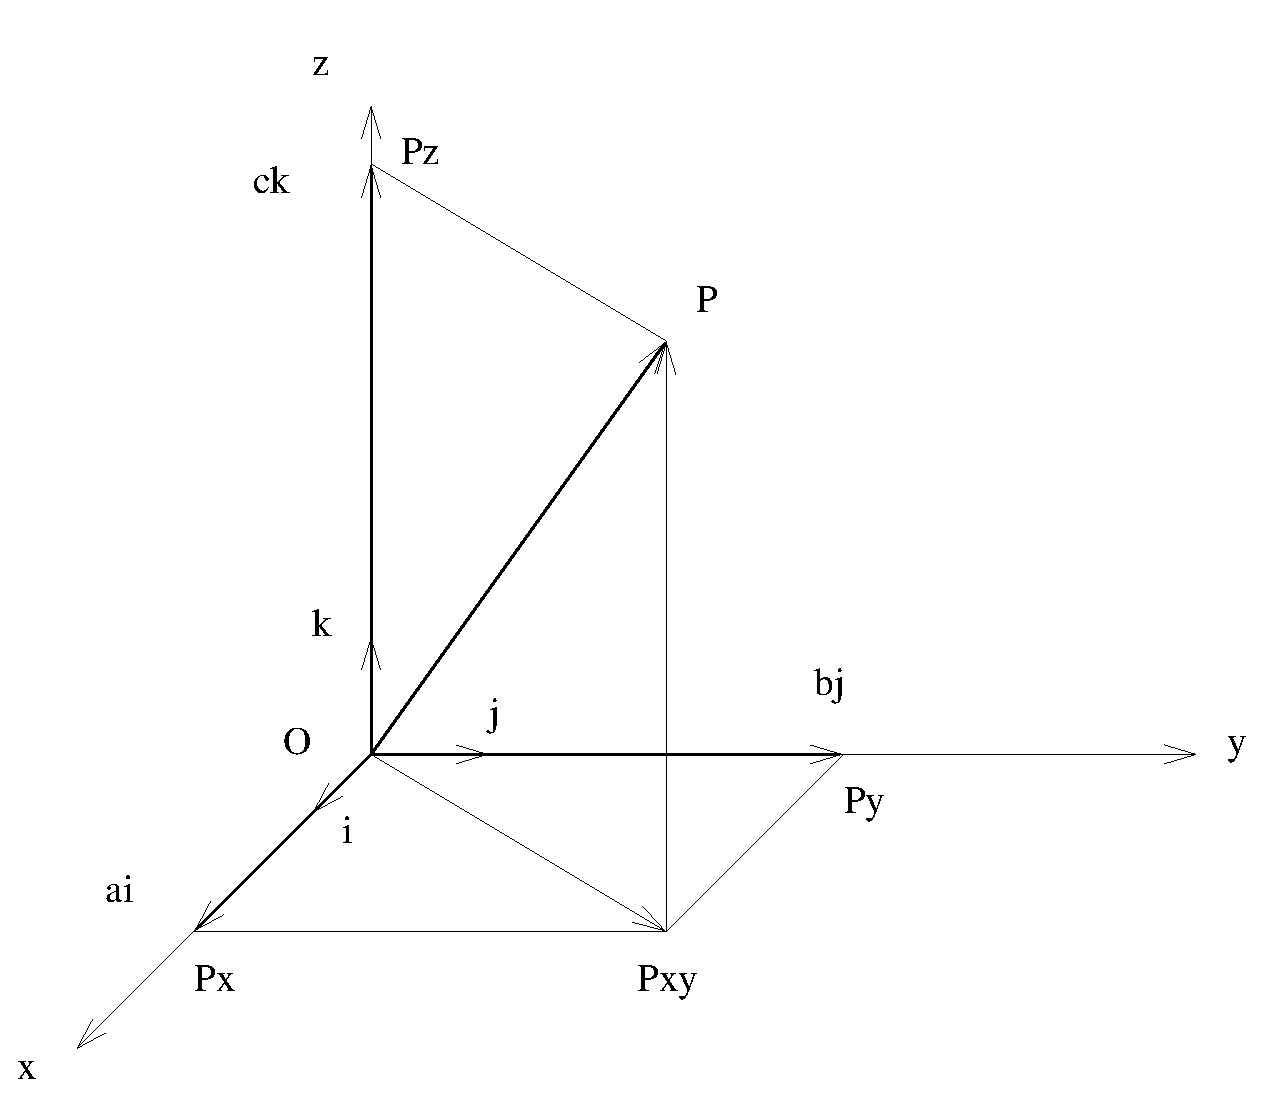
\includegraphics[height=2in]{../images/ok-vector_decomposition.eps}
  %\caption{Coordinates of a vector}
\end{figure}
%
$$\textbf{OP} = a\textbf{i}+b\textbf{j}+c\textbf{k} = \langle a, b, c\rangle\; .$$

\end{frame}

\begin{frame}
\frametitle{Operations in Coordinates}

\begin{itemize}
 \item Magnitude:
%
$$|\langle a, b, c \rangle| = |OP| = \sqrt{a^2+b^2+c^2}$$
%
\item Addition:
%
$$\langle x_1,y_1,z_1 \rangle + \langle x_2, y_2,z_2\rangle = \langle x_1+x_2, y_1+y_2, z_1+z_2\rangle\; .$$
%
\item Scalar multiple:
%
$$c\langle x, y, z\rangle = \langle cx, cy, cz\rangle\; .$$
%
\item General displacement from $A(x_A, y_A, z_A)$ to $B(x_B, y_B, z_B)$:
%
$$\textbf{AB} = \textbf{AO} +\textbf{OB} = \textbf{OB} - \textbf{OA} = \langle x_B-x_A, y_B-y_A, z_B-z_A\rangle \; .$$
\end{itemize}

\end{frame}


\begin{frame}
 \frametitle{Work done by a constant force}

\only<1>{
\begin{figure}[h]
  \psfrag{F}{$\textbf{F}$}
  \psfrag{O}{$O$}
  \psfrag{P}{$P$}
  \psfrag{a}{$\alpha$}
  \psfrag{pvF}{$\textbf{proj}_{\bm{v}} \textbf{F}$}
  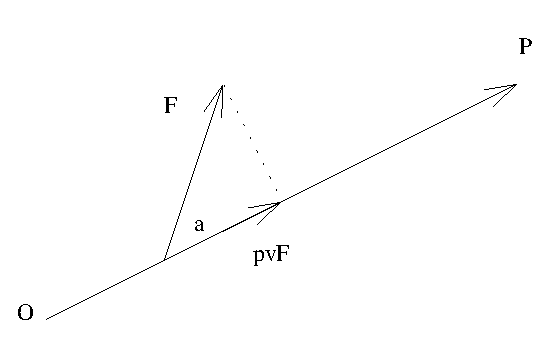
\includegraphics[height=2in]{../images/ok-positive_work.eps}
\end{figure}

$$W = |\textbf{proj}_{\bm{v}} \textbf{F}| \, |\textbf{OP}| =|\textbf{F}| \, |\textbf{OP}|\, \cos{\alpha}\; .$$}

\only<2>{
\begin{figure}[h]
  \psfrag{F}{$\textbf{F}$}
  \psfrag{O}{$O$}
  \psfrag{P}{$P$}
  \psfrag{a}{$\alpha$}
  \psfrag{pvF}{$\textbf{proj}_{\bm{v}} \textbf{F}$}
  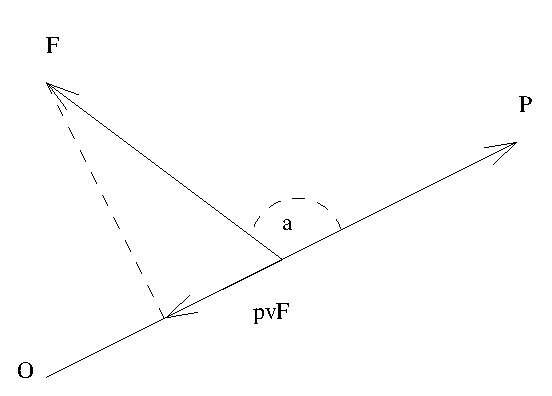
\includegraphics[height=2in]{../images/ok-negative_work.eps}
\end{figure}

$$W = - |\textbf{proj}_{\bm{v}} \textbf{F}| \, |\textbf{OP}| = |\textbf{F}| |\textbf{OP}| \cos{\alpha}\; .$$}

\end{frame}


\begin{frame}
 \frametitle{Dot Product}

\begin{figure}[h]
  \psfrag{u}{$\textbf{u}$}
  \psfrag{v}{$\textbf{v}$}
  \psfrag{a}{$\alpha$}
  \psfrag{pvu}{$\textbf{proj}_{\bm{v}} \textbf{u} = (comp_{\bm{v}} \textbf{u}) \hat{\textbf{v}}$}
  \psfrag{ovu}{$\textbf{orth}_{\bm{v}} \textbf{u}$}
  \psfrag{vh}{$\widehat{\textbf{v}}$} 
  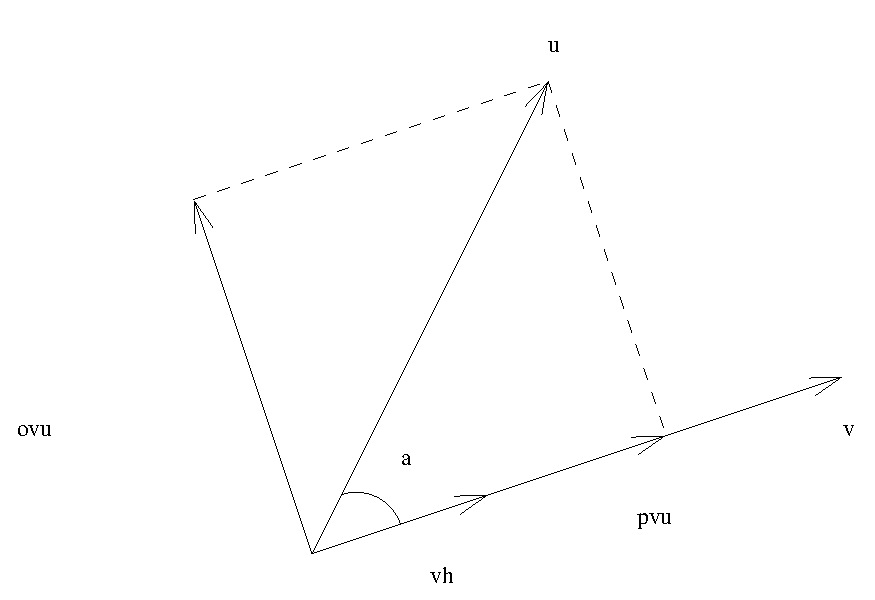
\includegraphics[height=1in]{../images/ok-dot_product.eps}
\end{figure}

\begin{itemize}
\item $\textbf{u}$, $\textbf{v}$ vectors, $\textbf{v}\neq \textbf{0}$.

\item $\textbf{proj}_{\bm{v}} \textbf{u}$: projection of $\textbf{u}$ along $\textbf{v}$;

  \item $\textbf{orth}_{\bm{v}} \textbf{u}$: projection of $\textbf{u}$ orthogonal to $\textbf{v}$;

  \item $\hat{\textbf{v}} = \frac{1}{|\textbf{v}|} \textbf{v}$: unit vector along $\textbf{v}$;

  \item $\textbf{proj}_{\bm{v}} \textbf{u} = (comp_{\bm{v}} \textbf{u}) \hat{\textbf{v}}$

  \item $comp_{\bm{v}} \textbf{u}$: scalar projection of $\textbf{u}$ onto $\textbf{v}$;

  \item Dot product of $u$ and $v$:
%
$$\textbf{u} \cdot \textbf{v} = (comp_{\bm{v}} \textbf{u}) \, |\textbf{v}|\; .$$
\end{itemize}

\end{frame}

\begin{frame}
 \frametitle{Properties of Dot Product}

  \begin{itemize}
   \item If $\textbf{v}=\textbf{0}$ or $\textbf{u}=\textbf{0}$, then $\textbf{u}\cdot \textbf{v} =0$.

  \item If $\textbf{u} \neq 0 \neq \textbf{v}$, then $comp_{\bm{v}} \textbf{u} = |\textbf{u}|\cos{\alpha}$
%
$$\textbf{u} \cdot \textbf{v} = |\textbf{u}| \, |\textbf{v}|\,\cos{\alpha}$$
%
\item If $\textbf{u}\neq \textbf{0} \neq \textbf{v}$, then
%
$$\textbf{u} \cdot \textbf{v} = 0 \Longleftrightarrow \textbf{u} \bot \textbf{v}\; .$$
%
\item $\textbf{u} \cdot \textbf{v} = (\textbf{proj}_{\bm{v}} \textbf{u}) \cdot \textbf{v}$

\item The dot product is linear in each argument:
%
$$ (a \textbf{u} + b \textbf{w}) \cdot \textbf{v} = a \textbf{u} \cdot \textbf{v} + b \textbf{w} \cdot \textbf{v}$$
%
$$ \textbf{u} \cdot (a \textbf{v} + b \textbf{w}) = a \textbf{u} \cdot \textbf{v} + b \textbf{u} \cdot \textbf{w}$$

\item Dot product is positive definite:
%
$$\textbf{v} \cdot \textbf{v} = |\textbf{v}|^2 \geqslant 0 \text{ and }
\textbf{v}\cdot \textbf{v} = 0 \leftrightarrow \textbf{v}=\textbf{0}$$
  \end{itemize}

\end{frame}

\begin{frame}
 \frametitle{Computations in Coordinates}

 \begin{itemize}
  \item  $Oxyz$: rectangular coordinate system

  \item $\textbf{i}$, $\textbf{j}$, $\textbf{k}$: unit vectors along fundamental directions.
%
$$ \textbf{i} \cdot \textbf{j} = \textbf{j} \cdot \textbf{i} = \textbf{j} \cdot \textbf{k}
 = \textbf{k} \cdot \textbf{j} = \textbf{i} \cdot \textbf{k} = \textbf{k} \cdot \textbf{i} = 0$$
%
$$\textbf{i} \cdot \textbf{i} = \textbf{j} \cdot \textbf{j} = \textbf{k} \cdot \textbf{k} = 1$$

  \item $\textbf{u} = u_1 \textbf{i} + u_2 \textbf{j} + u_3 \textbf{k} = \langle u_1, u_2, u_3 \rangle$,
 $\textbf{v}=v_1 \textbf{i} + v_2 \textbf{j} + v_3 \textbf{k} = \langle v_1, v_2, v_3 \rangle$,
%
$$\textbf{u} \cdot \textbf{v} = \langle u_1, u_2, u_3 \rangle \cdot \langle v_1, v_2, v_3 \rangle =
u_1v_1 + u_2 v_2 +u_3 v_3\; .$$

\item Example: $\langle 1,2,3 \rangle \cdot \langle 6,5,4 \rangle = 1 \cdot 6 + 2\cdot 5 + 3 \cdot 4 = 28$.
 \end{itemize}
\end{frame}

\begin{frame}
  \frametitle{Projections in Coordinates}

$\textbf{u} = u_1 \textbf{i} + u_2 \textbf{j} + u_3 \textbf{k} = \langle u_1, u_2, u_3 \rangle$,
 $\textbf{v}=v_1 \textbf{i} + v_2 \textbf{j} + v_3 \textbf{k} = \langle v_1, v_2, v_3 \rangle$
%
$$comp_{\bm{v}} \textbf{u} = \frac{\textbf{u}\cdot \textbf{v}}{|\textbf{v}|} =
\frac{u_1v_1+u_2v_2+u_3v_3}{\sqrt{v_1^2+v_2^2+v_3^2}}$$
%
$$comp_{\langle 6,5,4\rangle} \langle 1,2,3\rangle = \frac{28}{\sqrt{77}}\; .$$
%
$$\hat{\textbf{v}} = \frac{1}{|\textbf{v}|} \textbf{v} =
\frac{1}{\sqrt{77}} \langle 6,5,4\rangle\; .$$

$$\textbf{proj}_{\bm{v}} \textbf{u} = \frac{\textbf{u} \cdot \textbf{v}}{|\textbf{v}|} \, \widehat{\textbf{v}} =
\frac{\textbf{u} \cdot \textbf{v}}{|\textbf{v}|^2} \, \textbf{v}\; .$$
%
$$\textbf{proj}_{\langle 6,5,4\rangle} \langle 1,2,3\rangle = \frac{28}{77} \langle 6,5,4\rangle\; .$$

$$\textbf{orth}_{\langle 6,5,4\rangle} \langle 1,2,3\rangle = \langle 1,2,3\rangle -
\textbf{proj}_{\langle 6,5,4\rangle} \langle 1,2,3\rangle$$

\end{frame}

\begin{frame}
 \frametitle{Angles}

$$\cos{\alpha} = \frac{\textbf{u} \cdot \textbf{v}}{|\textbf{u}|\, |\textbf{v}|} \to \alpha =
\arccos{\left( \frac{\textbf{u} \cdot \textbf{v}}{|\textbf{u}|\, |\textbf{v}|} \right)}$$

Example:

\bigskip

Angle between $\langle 1,2,3\rangle$ and $\langle 6,5,4\rangle$:
%
$$\alpha = \arccos{\left( \frac{28}{\sqrt{14}\, \sqrt{77}} \right)} =
\arccos{\left( \frac{4}{\sqrt{22}} \right)}$$

\end{frame}

\begin{frame}
 \frametitle{Direction Angles}

\begin{figure}[h]
  \psfrag{u}{$\textbf{u}$}
  \psfrag{i}{$\textbf{i}$}
  \psfrag{j}{$\textbf{j}$}
  \psfrag{k}{$\textbf{k}$}
  \psfrag{a}{$\alpha$}
  \psfrag{b}{$\beta$}
  \psfrag{c}{$\gamma$}
  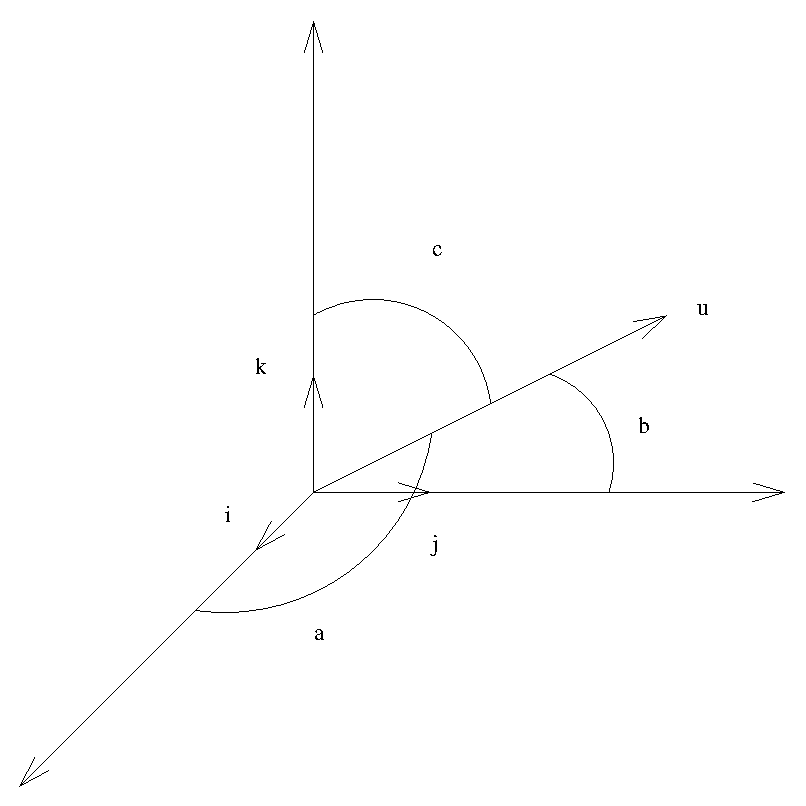
\includegraphics[height=2in]{../images/ok-direction_angles.eps}
\end{figure}


$\textbf{u} = \langle u_1, u_2, u_3\rangle, \qquad \alpha = \angle (\textbf{u},\textbf{i}) \qquad \beta =
\angle (\textbf{u},\textbf{j}) \qquad \gamma = \angle (\textbf{u},\textbf{k}) \; .$

$$\cos{\alpha} = \frac{\textbf{u} \cdot \textbf{i}}{|\textbf{u}|\, |\textbf{i}|} =
\frac{u_1}{\sqrt{u_1^2+u_2^2+u_3^2}}$$

Similar for $\cos{\beta}$ and $\cos{\gamma}$. Then:
%
$$\cos^2\alpha + \cos^2\beta + \cos^2\gamma = 1\; .$$

\end{frame}

\begin{frame}
 \frametitle{Rotational Effect}

 \begin{itemize}
  \item Rigid rod $OP$, fixed at $O$, $\textbf{r}=\textbf{OP}$. Force $\textbf{F}$ applied at $P$.
 \end{itemize}
%
\begin{figure}[h]
  \psfrag{F}{$\textbf{F}$}
  \psfrag{r}{$\textbf{r}$}
  \psfrag{O}{$O$}
  \psfrag{P}{$P$}
  \psfrag{}{$\alpha$}
  \psfrag{pfr}{$\textbf{proj}_{\bm{r}} \textbf{F}$}
  \psfrag{ofr}{$\textbf{orth}_{\bm{r}} \textbf{F}$}
  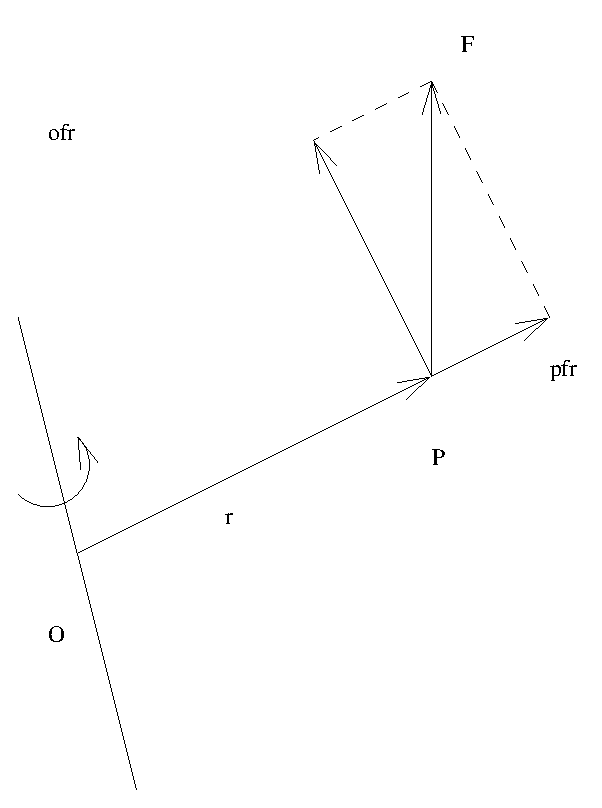
\includegraphics[height=1.5in]{../images/ok-torque.eps}
\end{figure}
%
\pause
\begin{itemize}
  \item $\textbf{proj}_{\bm{r}} \textbf{F}$: \pause no effect;
  \item $\textbf{orth}_{\bm{r}} \textbf{F}$: \pause rotational effect:\pause
  \begin{itemize}
    \item Axis of rotation: \pause perpendicular to $\textbf{r}$ and $\textbf{F}$;\pause
    \item Angular velocity: \pause proportional to $|\textbf{orth}_{\bm{r}} \textbf{F}|$;\pause
    \item Linear velocity: \pause proportional to $|\textbf{r}| \, |\textbf{orth}_{\bm{r}} \textbf{F}|$.
  \end{itemize}
\end{itemize}

\end{frame}

\begin{frame}
 \frametitle{Torque}

  Rotation in space $\Longleftrightarrow$ vector\pause
  \begin{itemize}
   \item Axis of rotation $\Longleftrightarrow$ Support of direction \pause
   \item Sense of rotation  $\Longleftrightarrow$ Direction of vector \pause
  \begin{itemize}
      \item Convention: Right Hand Rule\pause
  \end{itemize}
  \item Angular velocity $\Longleftrightarrow$ (proportional to) Magnitude of vector\pause
  \end{itemize}
\begin{center}
 $(\textbf{r}, \textbf{F}) \rightarrow$ rotation $\rightarrow$ vector = torque, $\bm{\tau}$
\end{center}



\begin{itemize}
 \item Support of direction: perpendicular to $\textbf{r}$ and $\textbf{F}$;
 \item Direction: Right Hand Rule;
 \item Magnitude: $|\bm{\tau}| = |\textbf{r}| \, |\textbf{orth}_{\bm{r}} \textbf{F}|$
\end{itemize}

\end{frame}

\begin{frame}
 \frametitle{Cross Product}

\begin{center}
 (\textbf{vector}, \textbf{vector}) $\to$ \textbf{vector}
\end{center}

\begin{figure}[h]
  \psfrag{u}{$\textbf{u}$}
  \psfrag{v}{$\textbf{v}$}
  \psfrag{ovu}{$\textbf{orth}_{\bm{u}} \textbf{v}$}
  \psfrag{a}{$\alpha$}
  \psfrag{uxv}{$\textbf{u} \times \textbf{v}$}
  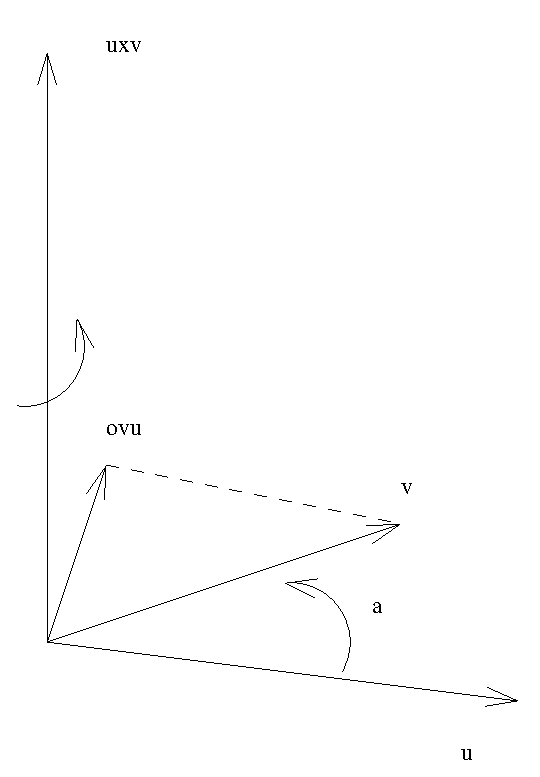
\includegraphics[height=1in]{../images/ok-cross_product.eps}
\end{figure}

\begin{itemize}
 \item If $\textbf{u}$, $\textbf{v}$ are non-zero and non-collinear vectors:\\
\begin{center}
 $\textbf{u} \times \textbf{v}$ is the vector determined by:
\end{center}
%
\begin{itemize}
 \item Support of direction of $\textbf{u} \times \textbf{v}$:
perpendicular to both $\textbf{u}$ and $\textbf{v}$;
 \item Direction of $\textbf{u} \times \textbf{v}$: given by Right Hand Rule;
 \item Magnitude of $\textbf{u} \times \textbf{v}$: product of $|\textbf{u}|$ and $|\textbf{orth}_{\bm{u}} \textbf{v}|$
%
$$|\textbf{u} \times \textbf{v}| = |\textbf{u}| \, |\textbf{orth}_u \textbf{v}| = |\textbf{u}| |\textbf{v}| \sin{\alpha}$$
%
\end{itemize}
\item If $\textbf{u}=\textbf{0}$ or $\textbf{v}=\textbf{0}$ or
$\textbf{u}$ and $\textbf{v}$ are collinear: \pause $\textbf{u} \times \textbf{v} = \textbf{0} $.
%
\end{itemize}

\end{frame}

\begin{frame}
 \frametitle{Properties of Cross Product}

$\textbf{u}$, $\textbf{v}$: non-zero vectors, $\alpha = \angle(\textbf{u},\textbf{v})$:
%
$$|\textbf{orth}_{\bm{u}} \textbf{v}| = |\textbf{v}|\sin\alpha
\Longrightarrow |\textbf{u} \times \textbf{v}| = |\textbf{u}| \, |\textbf{v}| \, \sin{\alpha}$$

Consequence: $|\textbf{v} \times \textbf{u}|  = | \textbf{u} \times \textbf{v}|$

\begin{itemize}
 \item \pause Cross product is anti-symmetric:
%
$$\textbf{v} \times \textbf{u} = - \textbf{u} \times \textbf{v} \; .$$
%
\item \pause Cross product is linear in each argument:
%
$$ \textbf{u} \times (a\textbf{v} + b\textbf{w}) =
a \textbf{u} \times \textbf{v} + b \textbf{u} \times \textbf{w}$$
%
$$(a\textbf{u} + b\textbf{w}) \times \textbf{v} =
a \textbf{u} \times \textbf{v} + b \textbf{w} \times \textbf{v}$$
\end{itemize}

\end{frame}

\begin{frame}
 \frametitle{Cross Product in Coordinates}

\begin{itemize}
 \item  $Oxyz$: rectangular coordinate system;
  \item $\textbf{i}$, $\textbf{j}$, $\textbf{k}$: unit vectors along fundamental directions.\pause
\end{itemize}
%
$$\textbf{i} \times \textbf{i} = \textbf{0} \quad , \quad \textbf{j} \times \textbf{j} =
\textbf{0} \quad , \quad \textbf{k} \times \textbf{k} = \textbf{0}$$
$$\textbf{i} \times \textbf{j} = \textbf{k} \quad , \quad \textbf{j} \times \textbf{k} =
\textbf{i} \quad , \quad \textbf{k} \times \textbf{i} = \textbf{j}$$
$$\textbf{j} \times \textbf{i} = -\textbf{k} \quad , \quad \textbf{k} \times \textbf{j} =
-\textbf{i} \quad , \quad \textbf{i} \times \textbf{k} = -\textbf{j}$$
\pause
If $\textbf{u} = u_1 \textbf{i} + u_2 \textbf{j} + u_3 \textbf{k} = \langle u_1, u_2, u_3 \rangle$,
 $\textbf{v}=v_1 \textbf{i} + v_2 \textbf{j} + v_3 \textbf{k} = \langle v_1, v_2, v_3 \rangle$:
%
$$\textbf{u} \times \textbf{v} = (u_1 \textbf{i} + u_2 \textbf{j} + u_3 \textbf{k})
\times (v_1 \textbf{i} + v_2 \textbf{j} + v_3 \textbf{k})= $$
%
$$= (u_2v_3 -u_3v_2) \textbf{i} + (u_3v_1-u_1v_3) \textbf{j} + (u_1v_2-u_2v_1) \textbf{k} \; .$$
\pause
$$\textbf{u} \times \textbf{v} = \langle u_1, u_2, u_3 \rangle \times \langle v_1, v_2, v_3 \rangle =
\left|  \begin{array}{ccc}
      \textbf{i} & \textbf{j} & \textbf{k} \\
      u_1 & u_2 & u_3 \\
      v_1 & v_2 & v_3
        \end{array}
\right|$$
\end{frame}

\begin{frame}
 \frametitle{Example}

$$\textbf{u} \times \textbf{v} = \langle u_1, u_2, u_3 \rangle \times \langle v_1, v_2, v_3 \rangle =
\left|  \begin{array}{ccc}
      \textbf{i} & \textbf{j} & \textbf{k} \\
      u_1 & u_2 & u_3 \\
      v_1 & v_2 & v_3
        \end{array}
\right|$$

If $\textbf{u} = \langle 1,2,3\rangle$ and $\textbf{v} = \langle 6,5,4 \rangle$, then
%
$$\textbf{u} \times \textbf{v} = \langle 1, 2, 3 \rangle \times \langle 6, 5, 4 \rangle =
\left|  \begin{array}{ccc}
      \textbf{i} & \textbf{j} & \textbf{k} \\
      1 & 2 & 3 \\
      6 & 5 & 4
        \end{array}
\right| = $$
%
$$= \left| \begin{array}{cc}
           2 & 3\\
	   5 & 4
          \end{array}
\right| \textbf{i} - \left| \begin{array}{cc}
           1 & 3\\
	   6 & 4
          \end{array}
\right| \textbf{j} + \left| \begin{array}{cc}
           1 & 2\\
	   6 & 5
          \end{array}
\right| \textbf{k}  = $$
%
$$=(2\cdot 4 -3\cdot 5) \textbf{i} - (1\cdot 4 - 3\cdot 6) \textbf{j} + (1 \cdot 5 - 2\cdot 6) \textbf{k} =$$
%
$$= -7 \textbf{i} + 14 \textbf{j} -7 \textbf{k} \; .$$
%
\end{frame}

\begin{frame}
 \frametitle{Applications of Cross Product}

\only<1>{Vector perpendicular to given vectors $\textbf{u}$ and $\textbf{v}$: $\textbf{u} \times \textbf{v}$.\\
Example: Vector perpendicular to $\textbf{u} = \textbf{i}+\textbf{j}$ and $\textbf{v}=\textbf{j}+\textbf{k}$:
%
\begin{align*}
 \textbf{w} = & (\textbf{i}+\textbf{j}) \times (\textbf{j}+\textbf{k}) =
\textbf{i} \times \textbf{j} + \textbf{i} \times \textbf{k} +
\textbf{j} \times \textbf{j} + \textbf{j} \times \textbf{k} = \\
 = & \textbf{k} -\textbf{j}+\textbf{0}+\textbf{i} = \textbf{i} - \textbf{j} + \textbf{k}\; .
\end{align*}}

\only<2->{$A$, $B$, $C$ points in space, $\textbf{u} = \textbf{AB}$, $\textbf{v}=\textbf{AC}$. Then \\
%
\begin{figure}[h]
  \psfrag{u}{$\textbf{v}$}
  \psfrag{v}{$\textbf{u}$}
  \psfrag{w}{$\textbf{w}$}
    \psfrag{A}{$A$}
    \psfrag{B}{$B$}
    \psfrag{C}{$C$}
    \psfrag{D}{$D$}
  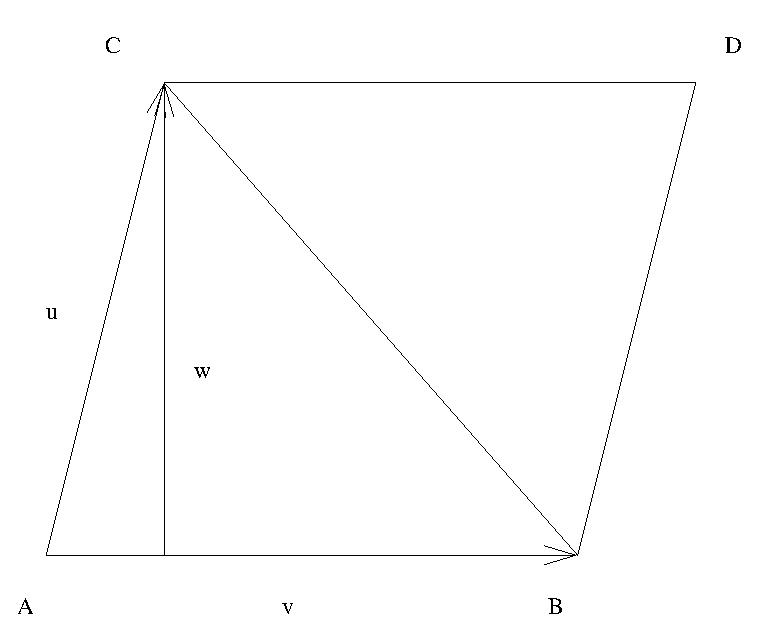
\includegraphics[height=1in]{../images/ok-area_triangle.eps}
\end{figure}
%
$$|\textbf{w}| = |\textbf{orth}_{\bm{u}} \textbf{v}| = \text{ distance from } C \text{ to } AB\; .$$
%
$$|\textbf{u} \times \textbf{v}| = |\textbf{orth}_{\bm{u}} \textbf{v}| \, |\textbf{u}| =
2 \text{area}(ABC) = \text{area}(ABDC)$$
%
$|\textbf{u} \times \textbf{v}|$ = Area of parallelogram on sides $\textbf{u}$ and $\textbf{v}$.
\pause

Example: Area of triangle $A(1,2,3)$, $B(2,3,1)$, $C(3,1,2)$
%
$$\text{Area}(ABC) = \frac{1}{2}|\textbf{AB} \times \textbf{AC}| =
\frac{1}{2}|\langle 1,1,-2\rangle \times \langle 2, -1, -1\rangle | = $$
%
$$= \frac{1}{2} |\langle -3, -3, -3 \rangle| = \frac{3\sqrt{3}}{2}\; .$$}

\end{frame}

\begin{frame}[label=current]
  \frametitle{Scalar Triple Product}

\begin{itemize}
 \item $A$, $B$, $C$, $D$ points in space;
  \item $\textbf{u} = \textbf{AB}$, $\textbf{v}=\textbf{AC}$, $\textbf{w}=\textbf{AD}$;
  \item $R=R(\textbf{u},\textbf{v},\textbf{w})$: box on sides $\textbf{u}$, $\textbf{v}$, $\textbf{w}$.\pause
%
\begin{figure}[h]
  \psfrag{u}{$\textbf{u}$}
  \psfrag{v}{$\textbf{v}$}
  \psfrag{w}{$\textbf{w}$}
  \psfrag{uxv}{$\textbf{u}\times \textbf{v}$}
  \psfrag{ow}{$\textbf{r}$}
  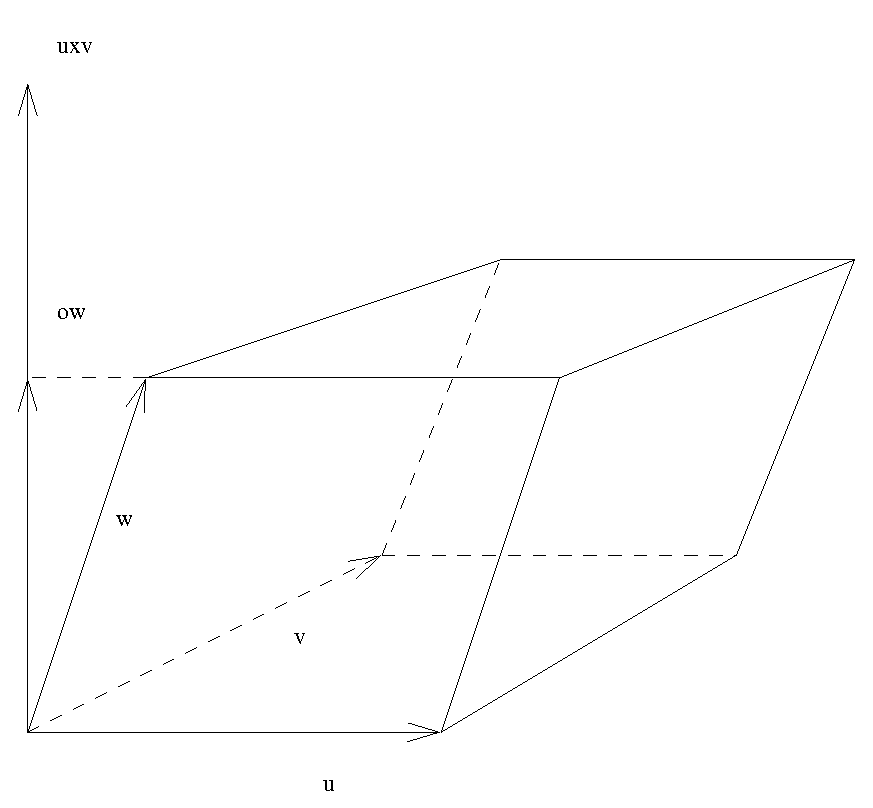
\includegraphics[height=1in]{../images/ok-volume_box.eps}
\end{figure}
%
$$\text{Vol}(R) = |\textbf{u} \times \textbf{v}| |\textbf{r}| = |\textbf{u} \times \textbf{v}| \, |\textbf{proj}_{\bm{u} \times \bm{v}} \textbf{w}| =
|\textbf{w} \cdot (\textbf{u} \times \textbf{v})|\; .$$
%
\item $\textbf{w} \cdot (\textbf{u} \times \textbf{v})$: scalar triple product.

\item If $\textbf{u} =\langle u_1,u_2,u_3\rangle$,
$\textbf{v} =\langle v_1,v_2,v_3\rangle$, and $\textbf{w} =\langle w_1,w_2,w_3\rangle$, then
%
$$\textbf{w} \cdot (\textbf{u} \times \textbf{v}) = \left|
\begin{array}{ccc}
w_1 & w_2 & w_3 \\
u_1 & u_2 & u_3 \\
v_1 & v_2 & v_3
\end{array}
 \right|$$
\end{itemize}

\end{frame}

\begin{frame}
  \frametitle{Orientations of Space}

\begin{itemize}
 \item The following are equivalent:
\begin{itemize}
  \item Every vector in space can be decomposed along $\textbf{u}$, $\textbf{v}$, $\textbf{w}$;
  \item The box $R(\textbf{u},\textbf{v},\textbf{w})$ is non-degenerate;
  \item $Vol(R(\textbf{u},\textbf{v},\textbf{w})) \neq 0$;
  \item $\textbf{u} \cdot (\textbf{v} \times \textbf{w}) \neq 0$.
\end{itemize}
%
\item \pause If any of the above is valid: $\{ \textbf{u}, \textbf{v}, \textbf{w}\}$ is a frame.

\item Rectangular coordinate system $\to$ fundamental frame $\{ \textbf{u}, \textbf{v}, \textbf{w}\}$

\item Consistent Right Hand Rule ($\textbf{w}=\textbf{u} \times \textbf{v}$) if and only if
%
$$\textbf{u} \cdot (\textbf{v} \times \textbf{w}) >0$$
%
The frame $\{ \textbf{u}, \textbf{v}, \textbf{w}\}$ is positively oriented if
$\textbf{u} \cdot (\textbf{v} \times \textbf{w}) >0$
%
\end{itemize}

\end{frame}
